\chapter{Introduction}\label{sec:introduction}

\section{Quantum Bits}
\label{subsec:qubits}

INTRODUCE CONCEPT OF DROPPING GLOBAL PHASE SOMEWHERE!

\subsection{Single Qubit Systems}
\label{subsubsec:qubits}
%Classical computers manipulate bits and the quantum equivalent is called a quantum bit, often abbreviated as qubit.
Classical computers manipulate bits, whereas quantum computer's most fundamental unit is called a quantum bit, often abbreviated as qubit. Bits as well as qubits are binary entities, meaning they can only take the values 0 and 1. A classical non-probabilistic bit can only be in one of the two possible states at once. In contrast, qubits obey the laws of quantum mechanics, which gives rise to the powerful property that - besides being a definite 0 or 1 - they can also be in a superposition of the two states. Mathematically this is expressed as a linear combination of the states 0 and 1:
\begin{equation}
\label{equ: simplequbit}
\ket{q} = \alpha \ket{0} + \beta \ket{1}
\end{equation}
where $\alpha$ and $\beta$ are complex coefficients and are often referred to as phase factors. \0 is the Dirac notation for the qubit being in state 0 and it represents a two-dimensional vector in a complex 2-D vector space (called Hilbert space $\mathcal{H}_{2}$). \0 and \1 are the the computational basis states and they constitute an orthonormal basis of $\mathcal{H}_{2}$. For the sake of clarity, \0 and \1 can be thought of as the 2-D vectors shown below.
\begin{equation}
\label{equ: 0and1kets}
\ket{0} =  \colvec{1\\0} \quad \quad \ket{1} = \colvec{0\\1}
\end{equation}
However, even though a qubit can be in as superposition of \0 and \1, when measured it will take the value \0 with a probability of ${|\alpha|}^{2}$ and \1 with a probability of ${|\beta|}^{2}$. Since the total probability of measuring any value has to be 1, the following normalization condition must be satisfied:
\begin{equation}
\label{equ: normalization}
{|\alpha|}^{2} + {|\beta|}^{2} =  1
\end{equation}
Therefore, a qubit is inherently probabilistic but when measured it collapses into a single classical bit (0 or 1). It follows that a measurement destroys information about the superposition of the qubit (the values of $\alpha$ and $\beta$). This constitutes one of the main difficulties when designing quantum algorithms since only limited information can be obtained about the final states of the qubits in the quantum computer.

Using spherical polar coordinates, a single qubit can be visualized on the so-called Bloch sphere by parameterising $\alpha$ and $\beta$ in Equ.~\ref{equ: simplequbit} as follows:

\begin{equation}
\label{equ: blochqubit}
\ket{q} = \cos\frac{\theta}{2} \ket{0} + e^{i \phi} \sin\frac{\theta}{2} \ket{1}
\end{equation}

The Bloch sphere has a radius of 1 and is therefore a unit sphere. The \0 qubit state is defined to lie along the positive z-axis ($\hat{z}$) and the \1 state is defined to lie along the negative z-axis ($-\hat{z}$) as labelled in Fig.~\ref{fig:blochsphere}. At this point, it is important to note that these two states are mutually orthogonal in $\mathcal{H}_{2}$ even though they are not orthogonal on the Bloch sphere. 

Qubit states on the Bloch equator such as the $\hat{x}$ and $\hat{y}$ coordinate axes represent equal superpositions where \0 and \1 both have measurement probabilities equal to $0.5$. The $\hat{x}$-axis for example represents the equal superposition $\ket{q} = \frac{1}{\sqrt{2}} \ket{0} + \frac{1}{\sqrt{2}} \ket{1}$. As illustrated in Fig.~\ref{fig:blochsphere} any arbitrary 2-D qubit state $\ket{\psi}$ can be decomposed into the polar angles $\theta$ and $\phi$ and visualized as a vector on the Bloch sphere. Such an object is called the Bloch vector of the qubit state $\ket{\psi}$. The Bloch sphere will be the main visualization tool for qubit manipulations in this thesis.

\begin{figure}[!ht]
       \centering
       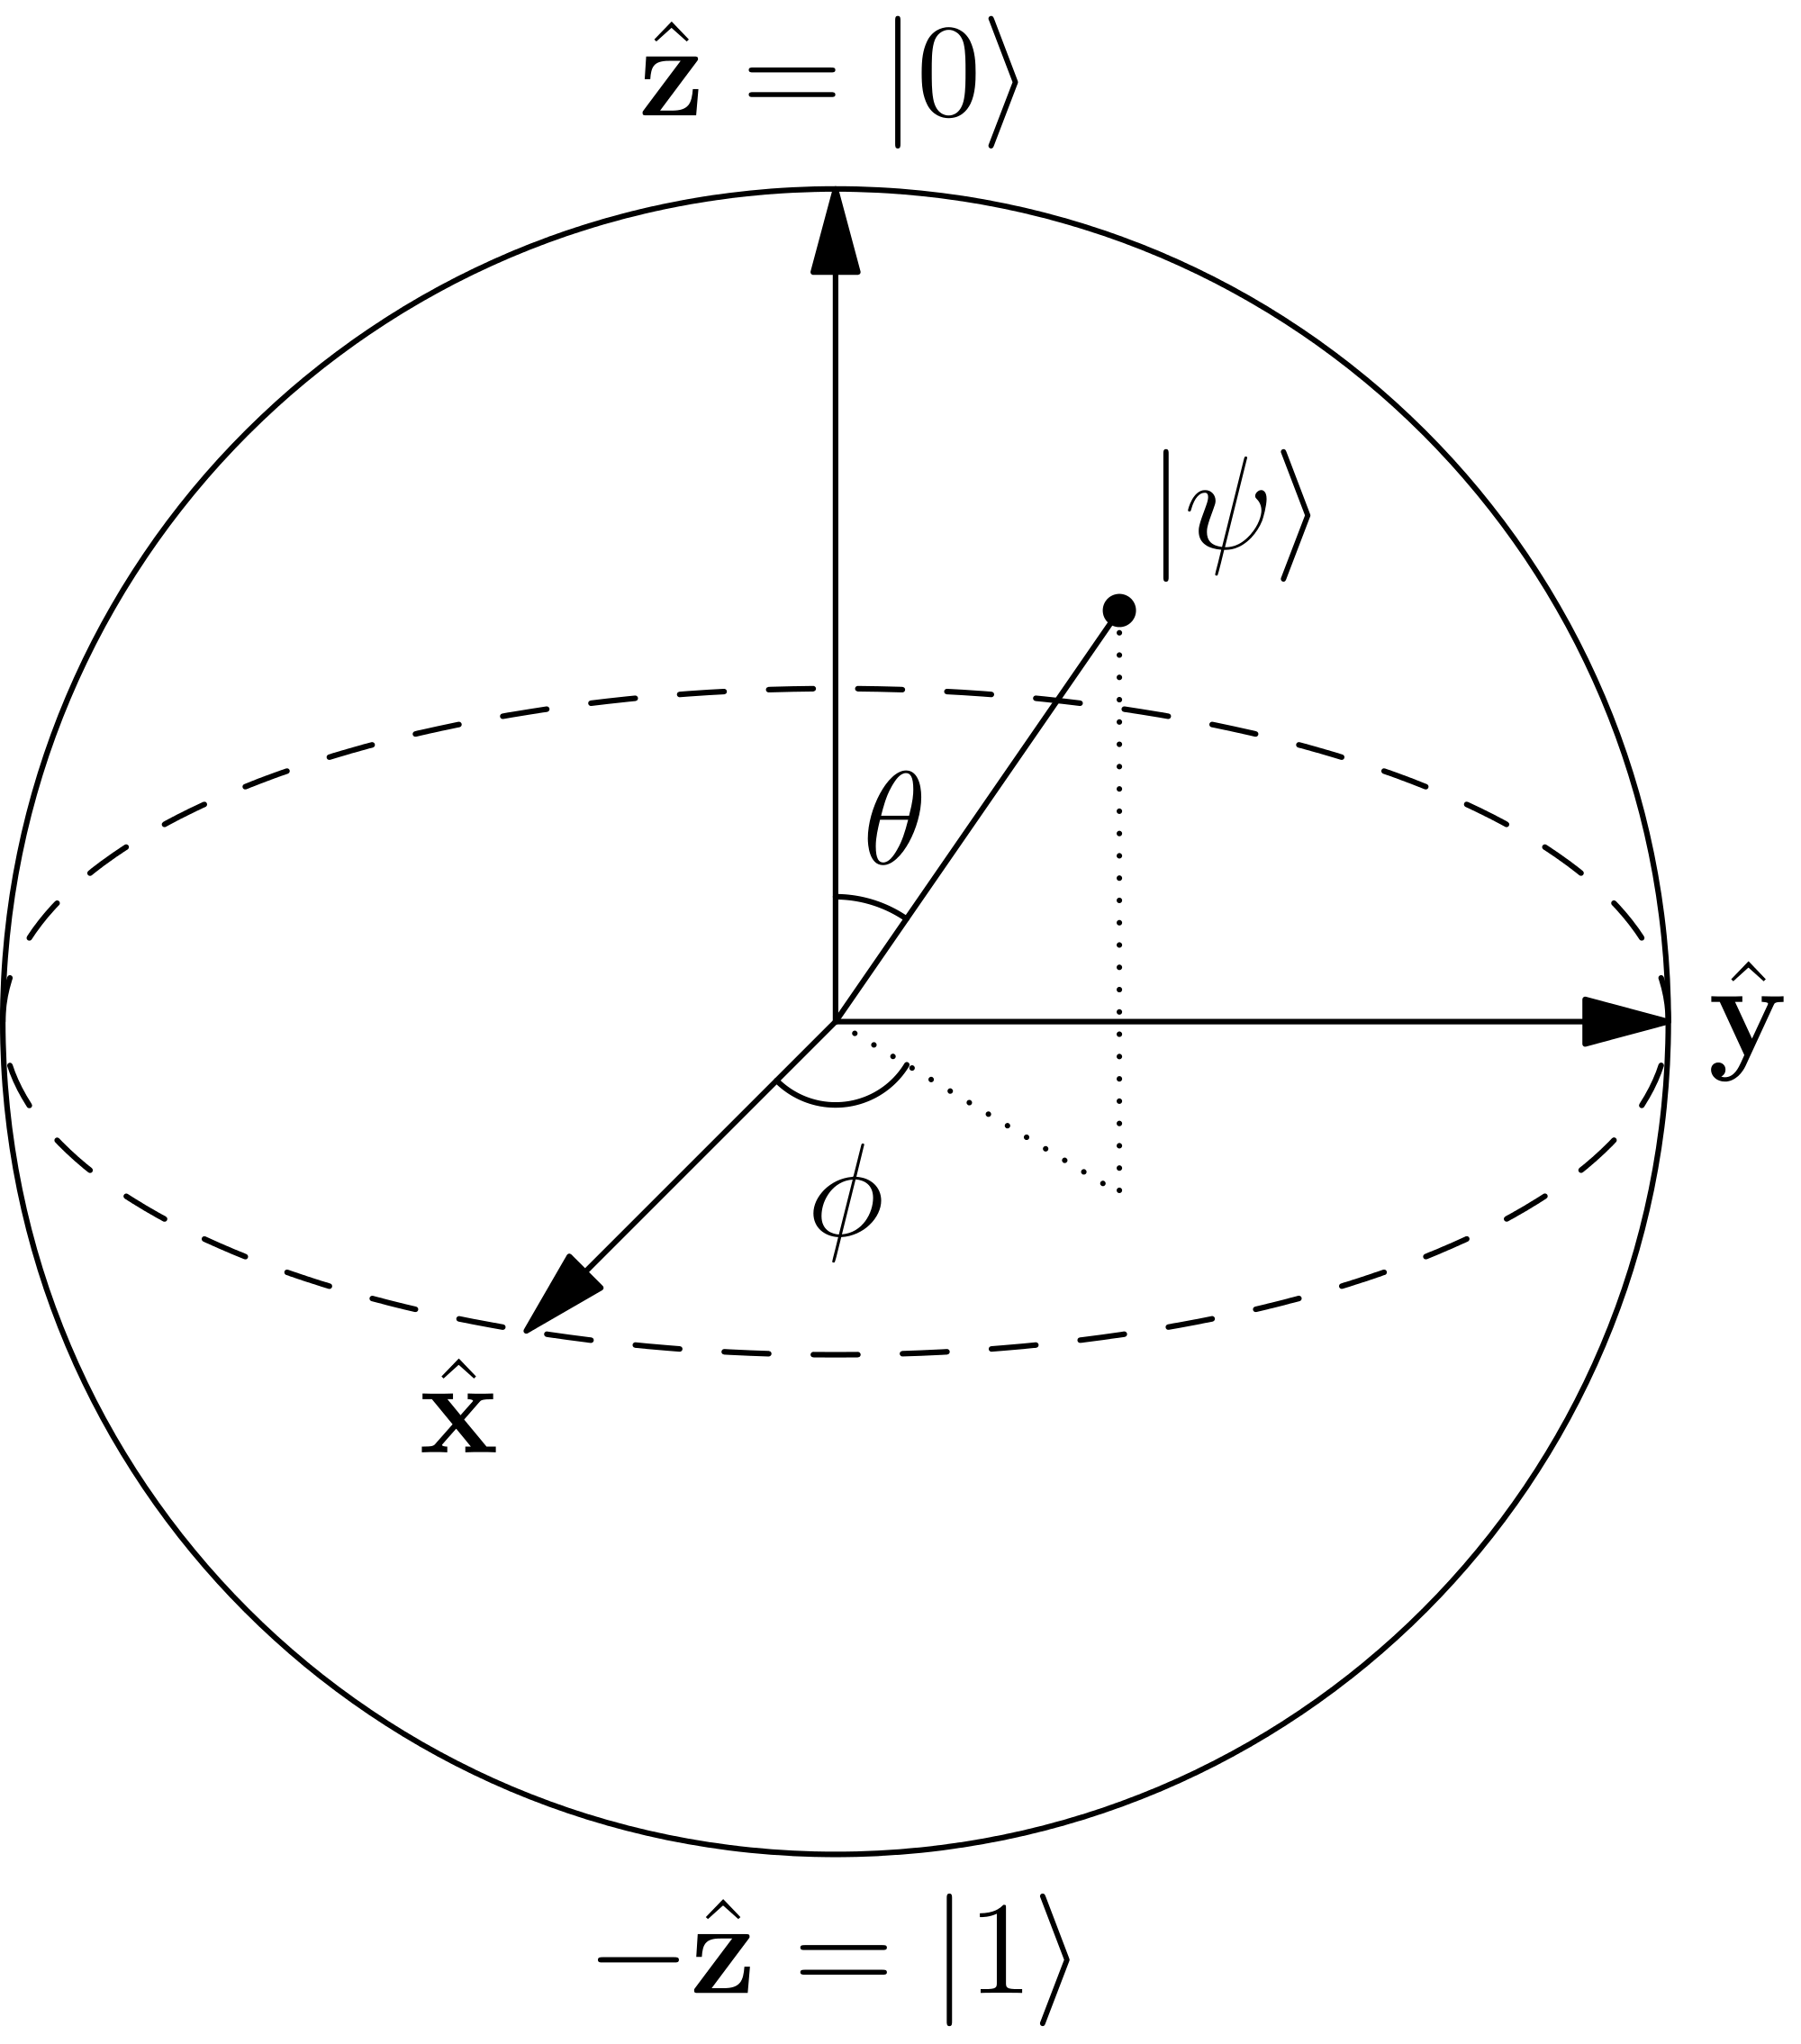
\includegraphics[scale=0.07]{img/blochsphere.png}
       \caption{\label{fig:blochsphere} An arbitrary two-dimensional qubit $\ket{\psi}$ visualized on the Bloch sphere.$^{1}$}
\end{figure}

\footnotetext[1]{Reprinted from Wikipedia, n.d., Retrieved September 7, 2016, from \url{https://en.wikipedia.org/wiki/Bloch_Sphere}. Copyright 2012 by Glosser.ca. Reprinted with permission.}

\subsection{Multiple Qubit Systems}
\label{subsec:multiplequbitsystems}

Introduce tensor products here!

\subsection{Entanglement}
\label{subsec:entanglement}

Introduce entanglement and non-factorising tensor states here!

%%%%% SECTION: Q LOGIC GATES


\section{Quantum Logic Gates}
\label{subsec:quantumlogicgates}
In order to perform quantum computations, tools, analogous to the classical logic gates, are needed for qubit manipulation. Quantum logic gates are square matrices that can be visualized as rotations on the Bloch sphere. The following subsections will introduce the major single and multi qubit logic gates.

\subsection{Single Qubit Gates}
\label{subsubsec:singlequbitgates}

ADD THE CIRCUIT REPRESENTATIONS OF THE RESPECTIVE GATES!

The four most basic single-qubit quantum gates are given by the four Pauli matrices listed below in Equ. ~\ref{equ: paulimatrices}.

\begin{align}
\label{equ: paulimatrices}
\sigma_{0} &= \mathbb{1} = \begin{pmatrix}
 1 & 0 \\ 
 0 & 1
 \end{pmatrix}
 \quad
 &&\sigma_{1} = \sigma_{x} = \begin{pmatrix}
 0 & 1 \\ 
 1 & 0
 \end{pmatrix}
 \nonumber
 \\
 \sigma_{2} &= \sigma_{y} = \begin{pmatrix}
 0 & -i \\ 
 i & 0
 \end{pmatrix}
 \quad
 &&\sigma_{3} = \sigma_{z} = \begin{pmatrix}
 1 & 0 \\ 
 0 & -1
 \end{pmatrix}
\end{align}

\subsubsection{Identity Gate}
\label{subsubsubsec:identitygate}

The simplest quantum gate is the identity or idle gate given by the 0\textsuperscript{th} Pauli matrix:

\begin{equation}
\sigma_{0} = \mathbb{1} = \begin{pmatrix}
 1 & 0 \\ 
 0 & 1
 \end{pmatrix}
\end{equation}

The action of a quantum gate on a qubit state can be analysed using the gate's matrix and the qubit's vector representation. Applying some straightforward linear algebra in this case yields:

\begin{equation}
\label{equ:identityverification}
\mathbb{1} \otimes (\alpha \ket{0} + \beta \ket{1}) = \begin{pmatrix}
 1 & 0 \\ 
 0 & 1
 \end{pmatrix} \begin{pmatrix}
 \alpha  \\ 
 \beta
 \end{pmatrix} = \begin{pmatrix}
 \alpha  \\ 
 \beta
 \end{pmatrix} = \alpha \ket{0} + \beta \ket{1}
\end{equation}

Hence, applying the identity gate to an arbitrary qubit state $\ket{q} = \alpha \ket{0} + \beta \ket{1}$ leaves the state unchanged as shown in Equ.~\ref{equ:identityverification}. The idle gate is mainly used for measuring the error and lifetimes of qubits since it only evolves the qubit in time without actively rotating the Bloch vector.

\subsubsection{Qubit Flip (X) Gate}
\label{subsubsubsec:xgate}

The quantum equivalent of the classical NOT gate is called X gate and is given by the 1\textsuperscript{st} Pauli matrix:

\begin{equation}
\sigma_{1} = X = \begin{pmatrix}
 0 & 1 \\ 
 1 & 0
 \end{pmatrix}
\end{equation}

The action of the X gate is easily verified by performing some linear algebra,

\begin{equation}
\label{equ:xverification1}
X \otimes (\alpha \ket{0} + \beta \ket{1}) = \begin{pmatrix}
 0 & 1 \\ 
 1 & 0
 \end{pmatrix} \begin{pmatrix}
 \alpha  \\ 
 \beta
 \end{pmatrix} = \begin{pmatrix}
 \beta  \\ 
 \alpha
 \end{pmatrix} = \beta \ket{0} + \alpha \ket{1}
\end{equation}

Thus, applying the X gate to qubit state $\ket{q}$ swaps the amplitudes of \0 and \1. More specifically, applying X to the \0 state results in the \1 state,

\begin{equation}
\label{equ:xverification2}
X \otimes \ket{0} = \begin{pmatrix}
 0 & 1 \\ 
 1 & 0
 \end{pmatrix} \begin{pmatrix}
 1  \\ 
 0
 \end{pmatrix} = \begin{pmatrix}
 0  \\ 
 1 \end{pmatrix} =  \ket{1}
\end{equation}

And the \0 state is recovered when applying X again to the \1 state,

\begin{equation}
\label{equ:xverification3}
X \otimes \ket{1} = \begin{pmatrix}
 0 & 1 \\ 
 1 & 0
 \end{pmatrix} \begin{pmatrix}
 0  \\ 
 1
 \end{pmatrix} = \begin{pmatrix}
 1  \\ 
 0 \end{pmatrix} =  \ket{0}
\end{equation}

From Equ.~\ref{equ:xverification1},~\ref{equ:xverification2} and~\ref{equ:xverification3} it follows that X is its own inverse:
\begin{align}
XX &= \mathbb{1} \\
X &= X^{-1}
\end{align}

\subsubsection{Phase Flip (Z) Gate}
\label{subsubsubsec:zgate}

The phase flip gate, often called Z gate, is a quantum logic gate without classical equivalent. Its matrix representation is given by the 3\textsuperscript{rd} Pauli matrix:

\begin{equation}
\sigma_{3} = Z = \begin{pmatrix}
 1 & 0 \\ 
 0 & -1
 \end{pmatrix}
\end{equation}



\begin{equation}
\label{equ:yverification}
Z \otimes (\alpha \ket{0} + \beta \ket{1}) = \begin{pmatrix}
 1 & 0 \\ 
 0 & -1
 \end{pmatrix} \begin{pmatrix}
 \alpha  \\ 
 \beta
 \end{pmatrix} = \begin{pmatrix}
 \alpha  \\ 
 -\beta
 \end{pmatrix} = \alpha \ket{0} - \beta \ket{1}
\end{equation}

\subsubsection{Qubit and Phase Flip (Y) Gate}
\label{subsubsubsec:ygate}

The combined qubit and phase flip gate, also called Y gate, is a quantum logic gate without classical equivalent since it involves the complex number i. Its matrix representation is given by the 2\textsuperscript{nd} Pauli matrix:

\begin{equation}
\sigma_{2} = Y = \begin{pmatrix}
 0 & -i \\ 
 i & 0
 \end{pmatrix}
\end{equation}

\begin{equation}
\label{equ:yverification}
Y \otimes (\alpha \ket{0} + \beta \ket{1}) = \begin{pmatrix}
 0 & -i \\ 
 i & 0
 \end{pmatrix} \begin{pmatrix}
 \alpha  \\ 
 \beta
 \end{pmatrix} = \begin{pmatrix}
 -i\beta  \\ 
 i\alpha
 \end{pmatrix} = -i\beta \ket{0} + i\alpha \ket{1}
\end{equation}

\subsubsection{Hadamard (H) Gate}
\label{subsubsubsec:hadamardgate}

\begin{equation}
H = \begin{pmatrix}
 \frac{1}{\sqrt{2}} & \frac{1}{\sqrt{2}} \\ 
 \frac{1}{\sqrt{2}} & -\frac{1}{\sqrt{2}}
 \end{pmatrix}
\end{equation}

\subsubsection{Clifford (H,S,Sd) Gates}
\label{subsubsubsec:cliffordgates}

\begin{equation}
S = \sqrt{Z} = \begin{pmatrix}
 1 & 0 \\ 
 0 & i
 \end{pmatrix}
\end{equation}

\begin{equation}
S^\dagger = \begin{pmatrix}
 1 & 0 \\ 
 0 & -i
 \end{pmatrix}
\end{equation}

\subsubsection{Non-Clifford (T,Td) Gates}
\label{subsubsubsec:noncliffordgates}

\begin{equation}
T = \sqrt{S} = \begin{pmatrix}
 1 & 0 \\ 
 0 & e^{\frac{i\pi}{4}}
 \end{pmatrix}
\end{equation}

\begin{equation}
T^\dagger = \begin{pmatrix}
 1 & 0 \\ 
 0 & e^{-\frac{i\pi}{4}}
 \end{pmatrix}
\end{equation}


%%%%% SUBSECTION: MULTIPLE Q LOGIC GATES


\subsection{Multiple Qubit Gates}
\label{subsubsec:multiqubitgates}

\subsubsection{Controlled NOT Gate}
\label{subsubsubsec:cnotgate}

\begin{equation}
CNOT = \begin{pmatrix}
 \mathbb{1} & 0 \\ 
 0 & X
 \end{pmatrix} = \begin{pmatrix}
 1 & 0 & 0 & 0 \\ 
 0 & 1 & 0 & 0 \\
 0 & 0 & 0 & 1 \\
 0 & 0 & 1 & 0 \\
 \end{pmatrix}
\end{equation}

\subsubsection{Toffoli Gate}
\label{subsubsubsec:toffoligate}

\begin{equation}
Toffoli = CCNOT = \begin{pmatrix}
 \mathbb{1}_6 & 0 \\ 
 0 & X
 \end{pmatrix} = \begin{pmatrix}
 1 & 0 & 0 & 0 & 0 & 0 & 0 & 0 \\ 
 0 & 1 & 0 & 0 & 0 & 0 & 0 & 0 \\ 
 0 & 0 & 1 & 0 & 0 & 0 & 0 & 0 \\ 
 0 & 0 & 0 & 1 & 0 & 0 & 0 & 0 \\ 
 0 & 0 & 0 & 0 & 1 & 0 & 0 & 0 \\ 
 0 & 0 & 0 & 0 & 0 & 1 & 0 & 0 \\
 0 & 0 & 0 & 0 & 0 & 0 & 0 & 1 \\ 
 0 & 0 & 0 & 0 & 0 & 0 & 1 & 0 \\ 
 \end{pmatrix}
\end{equation}

where $\mathbb{1}_6$ is the 6x6 identity matrix.

\subsubsection{Controlled U Gate}
\label{subsubsubsec:controlledugate}

\begin{equation}
CU = \begin{pmatrix}
 \mathbb{1} & 0 \\ 
 0 & U
 \end{pmatrix}
\end{equation}

%%%%% SECTION: MEASUREMENTS

\section{Qubit Measurements}
\label{subsec:qubitmeasurements}

\subsection{Standard Basis Measurement}
\label{subsubsec:standardbasismeasurement}

\subsection{Bloch Measurement (?)}
\label{subsubsec:blochmeasurement}

%%%%% SECTION: MACHINE LEARNING

%\section{Machine Learning}
%\label{subsec:machinelearning}

\section{Classical Machine Learning}
\label{subsec:classicalmachinelearning}

\subsection{k-nearest Neighbour Algorithm}
\label{subsubsec:knearestneighbour}

\section{Quantum Machine Learning}
\label{subsec:quantummachinelearning}

\subsection{Quantum k-nearest Neighbour Algorithm}
\label{subsubsec:quantumknearestneighbour}